\chapter{Modelling memory in language acquisition}

In this chapter, we describe the work we did in the context of an internship at the private company Lingvist Technologies during May-July 2017. The main product of the company is a computerised language learning tool that allows users to practice vocabulary in a foreign language in a dynamic online setting using spaced repetition.

The product has over~$10^6$~users learning several languages, thereby presenting a rich dataset where techniques of computer-assisted education can be tested and improved. Taking into account the population of users, statistical learning can be used to optimize the contents of the course based on models of learning and of users.

Our main contribution in this project was developing a data-driven model based on machine learning (ML) that estimates the prior vocabulary knowledge of users based on a small set of probe questions and the overall statistical properties of the user population. 

In this chapter, we will describe the problem of vocabulary prediction, give an overview of the model and validate it with respect to data. We discuss also the reference model that we formalized and the metrics that we developed to compare the improved model to the reference. We have found that the ML-based model improved over the existing prediction algorithm by about 40\% in terms of prediction efficiency, such that this algorithm was further put into production.

\section{Introduction}
It has been shown that individual tutoring can improve the results of average students by up to two standard deviations~\cite{corbett2001cognitive}. However, access to high-quality individual tutoring is limited, therefore using computerised assistants presents an opportunity to make learning more accessible. In a computerised learning course, tailoring the course contents to the specific pre-existing knowledge of an individual learner allows the learning material to be covered more efficiently by focussing on subjects that are not yet well understood as opposed to subjects that the learner (user) is likely to know well. Knowledge estimation deals with the question of parametrising and modelling the knowledge about various topics or items on a per-user basis. 

We describe a computational method for estimating the overall second-language vocabulary of users, based on answers to a small set of trial words that the users attempt to guess. Effectively, users entering the learning environment are presented with words in their target language, for which they provide their best answer. An example is shown on~\cref{fig:lu_example}. Such user-word-answer tuples form the basic unit of data in the learning environment.

\begin{figure}
\centering
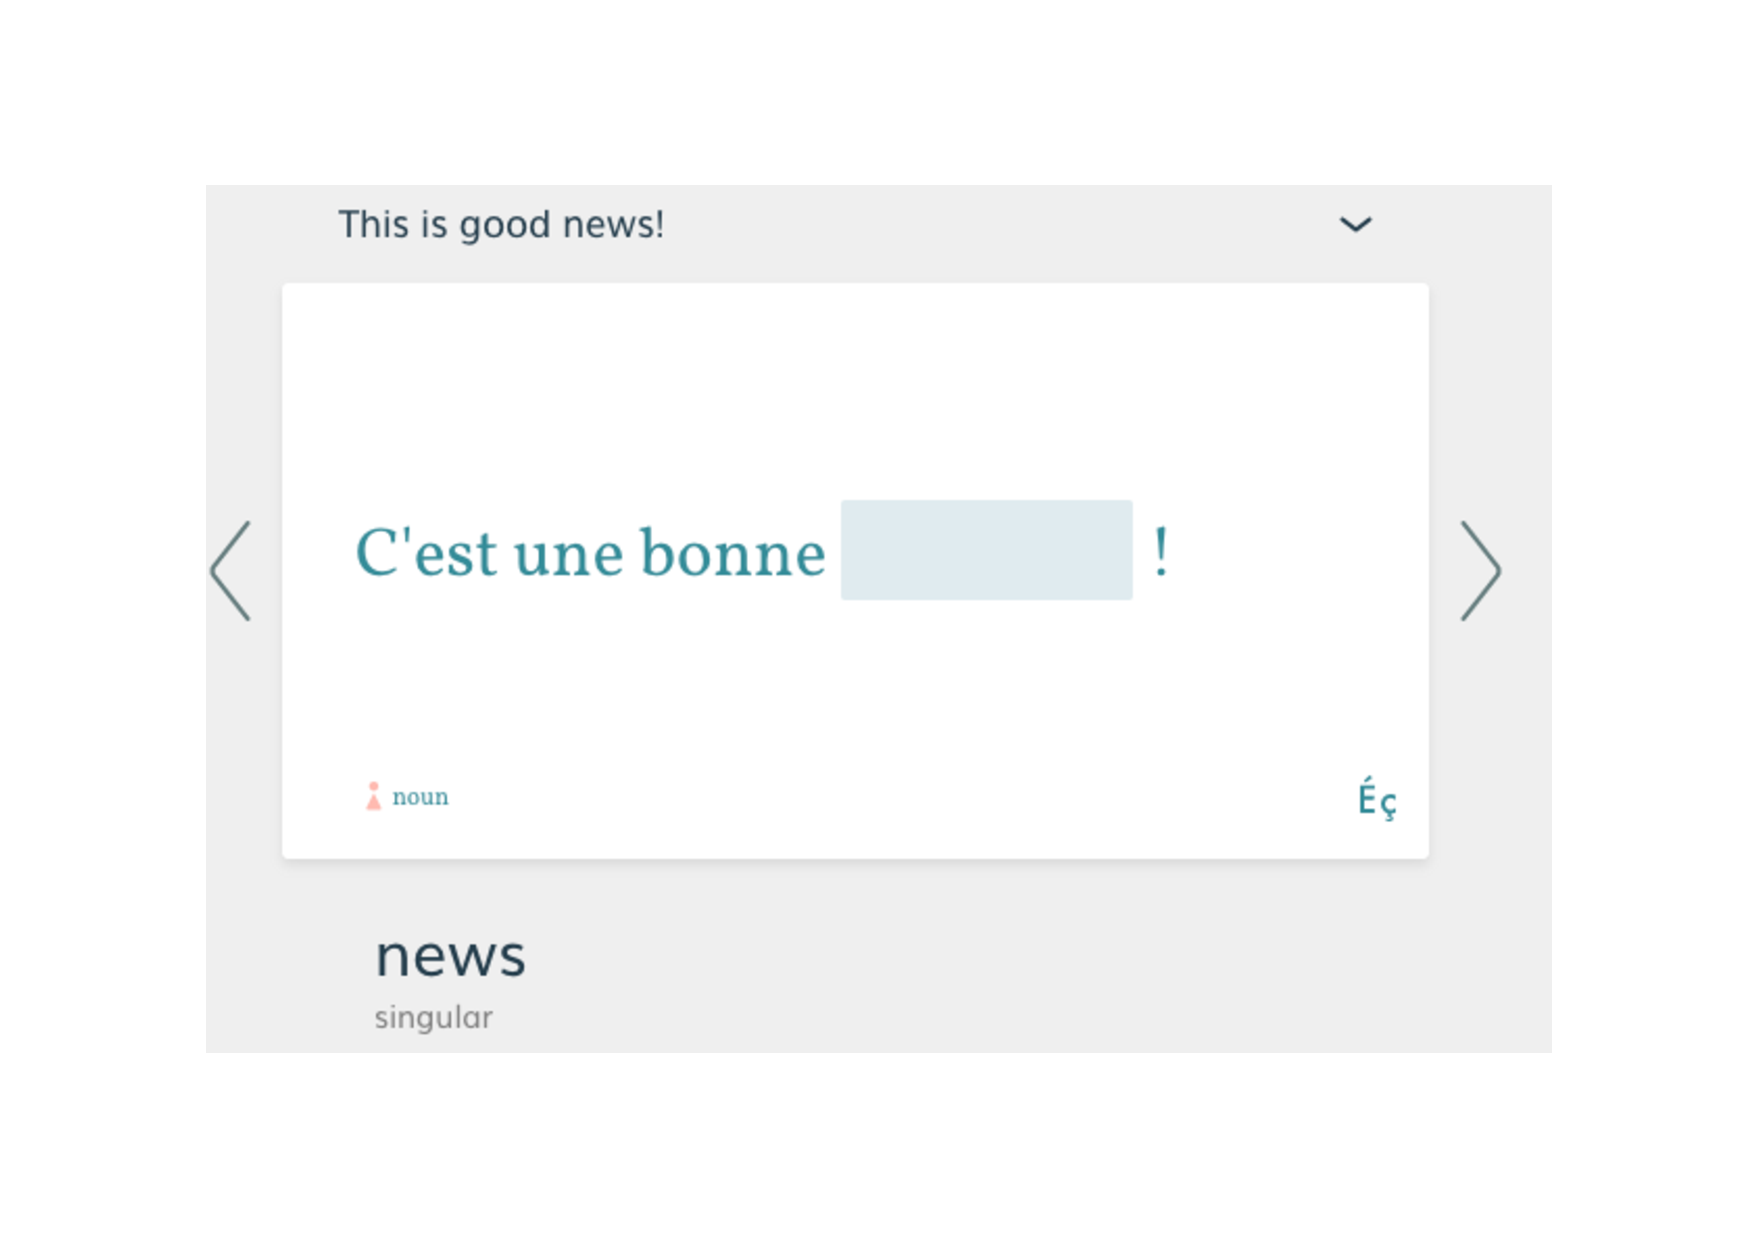
\includegraphics[width=0.6\linewidth]{figures/lingvist/example_lu.pdf}
\caption[An example exercise in the Lingvist environment]{An example of an exercise in the Lingvist environment, where the user is learning French based on English.} 
\label{fig:lu_example} 
\end{figure} 

By implementing a simplified version of Deep Knowledge Tracing~(DKT)~\cite{DBLP:journals/corr/PiechSHGSGS15}, we show that by predicting the knowledge of individual items on a per-user basis using a sequence of previous guesses, we can develop an accurate estimation procedure for the overall vocabulary knowledge of the user. We achieve this by compressing the sparse and variable-length guess sequences into a fixed-size representation using a recurrent neural network~(RNN) and furthermore mapping this small fixed-size representation into a vector that can be interpreted as distinct per-item knowledge likelihoods.

This chapter is organised as follows: in the first section, we review the mathematical background of the problem of knowledge estimation and present a statistical overview of the data. In the second section, we discuss the details of the RNN model that will be used to estimate the user knowledge and compare it with other models. In the third section, we summarise the studies that were made in optimizing the RNN model, analyse the results and discuss possible improvements that could be made to the model.

\section{Problem statement and data description}
In the following section, we will describe the problem of estimating the users' vocabulary knowledge in terms of guess likelihoods for basic language items and describe the dataset based on which we will construct the prediction model.

\subsection{Knowledge estimation}
The problem of knowledge estimation can formally be stated as follows. We have a set of items, indexed by~$n = {1, 2, \dots, N}$, for which users, indexed by~$m  = {1, 2, \dots, M}$~provide guesses which can be correct or incorrect, denoted by~$g_{nm}=\{1, 0\}$. Therefore on a per-user basis, the guess data form a sequence

$$S_m = [(n_1, g_1), \dots, (n_i, g_i), \dots, (n_T, g_T)]$$
where~$T$~is the number of guesses a user has made. The individual knowledge of a specific user~$n$~can then be succinctly written as~$\vec{g}_n = (g_1, g_2, \dots, g_M)$. We assume that we have no control over the order in which items are presented to the user, in general, the sequence may contain guesses in an arbitrary order, possibly with gaps between the successive indices~$m_i$~and~$m_{i+1}$.

\subsubsection{Lexical unit}
The items in the guess sequence themselves may be arbitrary, but in our case, they always represent word pairs, asking the user to guess a word in their target language based on an explanation in their source language. We use the term \textit{lexical unit} (LU) to denote such word pairs. An example LU would be the pair \textit{advice} - \textit{le conseil} in the English-French language pair, embedded as a completion in a sentence such as: \textit{Cette un bon~$\dots$~(advice)}.

These data can be represented as a~$(N \times M)$~matrix~$\mathbb{G} = (g_{nm})$, with~$N$~being the total number of users and~$M$~the total number of items. In general, users may answer questions from a randomized LU sequence, thus, this matrix is sparsely filled, as can be seen on~\cref{fig:user_data}, where we have shown the guess data for a small subset of users and LUs.

\begin{figure}[ht]
\centering
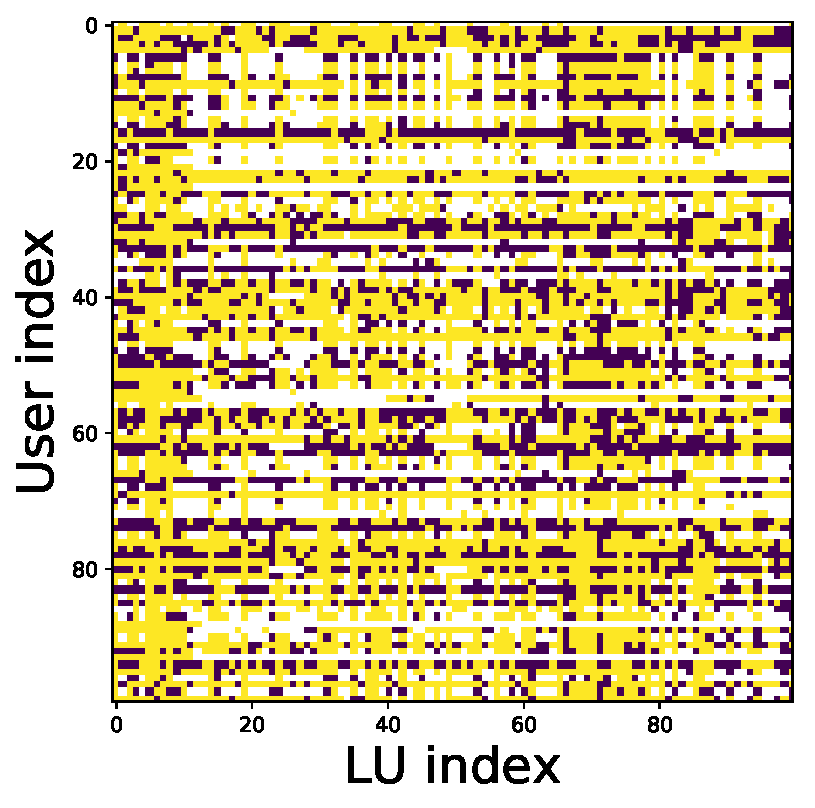
\includegraphics[width=0.5\linewidth]{figures/lingvist/user_data.pdf}
\caption[Word pair (LU) guess data for a subset of users and words]{Guess data for the first 100 users and the first 100 LUs, a small subset of the full user population and LU space. Correct guess attempts are shows as a yellow pixel, incorrect attempts where the users guess did not correspond to the correct answer with a brown pixel. Cases where data was not available are shown as white pixels. The relative sparsity of data results from the question algorithm sampling the LU space in a pseudo-random fashion.} 
\label{fig:user_data} 
\end{figure} 

\subsubsection{Prediction task}
The task of knowledge estimation is then to predict the guess probabilities~$\vec{g}_n$~for all items for an individual user~$n$, given a short ($\sim5\%$~of the total or about 10-50 guesses) subsequence of that user's guesses. This can further be seen in the context of knowledge tracing, where given a sequence of observations about a user~$\mathbf{x}_0 \dots \mathbf{x}_t$~over time steps~$t$, the task is to predict properties of the interaction~$\mathbf{x}_{t+1}$. Here, the interaction is formally a pair~$\mathbf{x}_t = \{n_t, g_t\}$~of the knowledge item and the guess. Time-dependent prediction is important for modelling the memory and learning capacity of users. In the studies that follow, we decoupled the study of time-dependent properties of learning from the initial knowledge, focusing on optimizing the method for predicting the pre-existing vocabulary.

The guess probabilities of items may be related to each other, such that knowing a difficult word would be a good predictor of knowing other words of similar difficulty. Therefore, the task is to model the full probability distribution~$p(\vec{g})$. However, we do not have an explicit labelling of which items are related and we hope to capture the essential properties of the knowledge probability by using the data directly.

\begin{figure}[ht]
\centering
\begin{tabular}{cc}
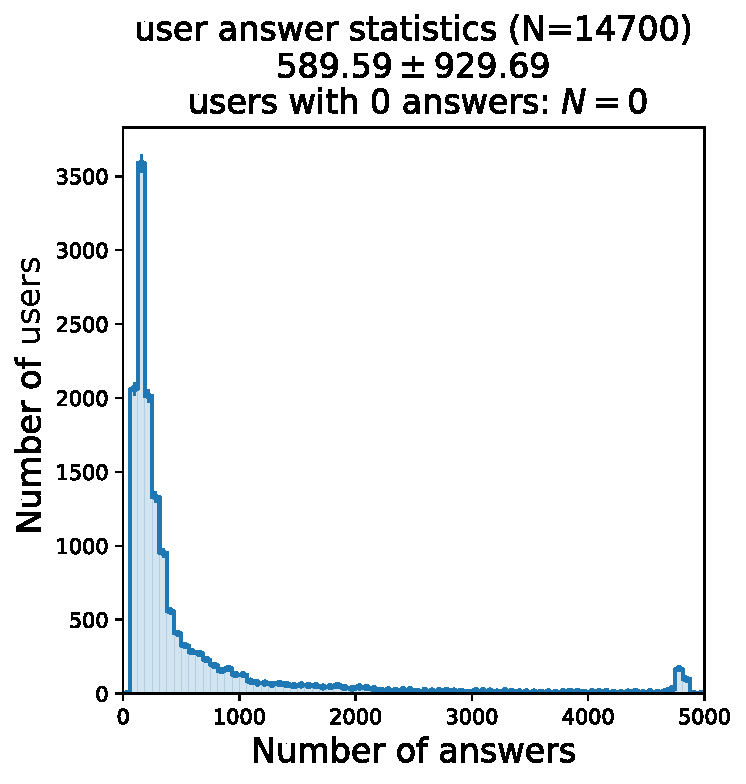
\includegraphics[width=0.5\linewidth]{figures/lingvist/user_answer_distribution.pdf} &
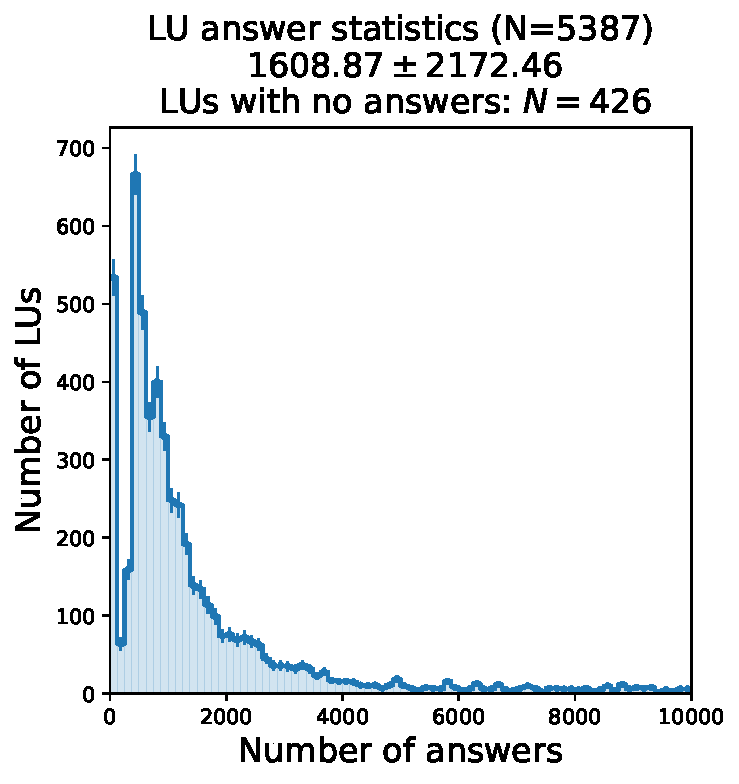
\includegraphics[width=0.5\linewidth]{figures/lingvist/lu_answer_distribution.pdf} \\
\end{tabular}
\caption[Distributions of guesses by LU and user]{On the left, we show the distribution of users by number of answered LUs. We have required that a user has answered at least 100 LUs. On the right, we show the corresponding distribution of LUs by number of answers from users. At this stage, LUs have not been filtered, hence the whole course is considered.} 
\label{fig:user_lu_distribution} 
\end{figure} 

\subsection{Data}
We use guess data for about 6 months between January - June 2017 from roughly 15000 users from the English to French course at Lingvist, requiring that users have answered at least 100 LUs. This corresponds to about 10 million user - guess pairs. The course consists of roughly 5400 individual LUs. Overall, an average user has answered about 590 LUs and an average LU has about 1600 answers, and the distributions follow a rough power law form, as can be seen on~\cref{fig:user_lu_distribution}. Although we used the English-French language pair for the primary studies, we have also validated the model on several other language pairs with less data, namely Russian-French, English-Taiwanese and English-German, and have seen that the results are broadly replicable.

The problem of predicting the properties of the guess matrix~$\mathbb{G}$~as stated here is well known in literature as matrix completion~\cite{candes2009exact}, where the task is to discover hidden or latent variables that would allow the unspecified elements of a matrix to be estimated based on assumptions about rows or columns being sampled from a common distribution. Such problems are typically solved with some combination of collaborative filtering and matrix factorization. However, as in the future we may also want to model time-dependent behaviour of the estimated knowledge, we seek a more generic solution to the problem that would make it possible to add arbitrary information about users and guesses and derive the appropriate model without much expert knowledge. Furthermore, in the future, the definition of a lexical unit (LU) may be expanded to encompass more general exercises beyond word pair guesses, for which a simple matrix representation may not be sufficiently flexible. 

\section{Model description}

\subsection{Reference models}

In this section we describe the baseline models that will be used as reference implementations to estimate the improved performance from the proposed approach. The simplest model for predicting the prior knowledge rate of words would simply be to assume that any user is an average user and each word with index~$n=1 \dots N$~has a probability~$p_n$~of being known by any user, where the probability is simply estimated by computing the ratio of correct to all guesses of this word by all users. Clearly this does not allow the learning experience to be tailored, but it is a reasonable first guess about the user in the absence of other data.

As the user proceeds through the course, their guesses will allow us to update our estimation of their knowledge in a Bayesian framework. In general, Bayesian Knowledge Tracing~\cite{corbett1994knowledge} has been shown to perform at least as well as the best machine-learning based models, however, such models require considerable domain knowledge and manual item labelling to be used successfully~\cite{khajah2016deep}, thus we investigate supervised neural networks as a possible solution.

In order to measure how well a model is able to predict user knowledge, we need to establish a set of metrics. In particular we use the number of correctly predicted items that the user actually knows (true positives) and the number of items incorrectly predicted to be known (false positives). Thus, we effectively treat the problem as binary classification with each guess attempt being an independent trial of equal weight.

We use these true and false positive rates to construct the receiver operating characteristic area-under curve (ROC AUC) metric as an overall average performance indicator. Such a metric considers all trials as equal, meaning it is tuned to measure the performance of the model on the same distribution of LUs that is used in the optimization. This is referred to as the trial-weighted case. An alternative would be to treat each LU, regardless of how many guesses have been made for it, as equal, effectively reducing the weight of the LUs for which very many users have provided guess data. We refer to this later as the LU-weighted case.

\subsection{Machine learning model}
\label{sec:nlp_model}
Since we may want to make predictions continuously as the user progresses through the course, the model should be able to deal with sequence data of varying length. This leads us to consider recurrent neural networks as a possible model architecture. In particular, inspired by the Deep Knowledge Tracing framework~\cite{DBLP:journals/corr/PiechSHGSGS15}, we use a Long Short-Term Memory (LSTM)~\cite{gers1999learning} architecture to summarize a guess history of arbitrary length as a vector of fixed length. The advantage of the LSTM-type model over standard RNN-s is that the network is augmented with a memory cell and gates for storing and forgetting the item in memory. This has been shown to help solve the vanishing gradient problem typical in RNN applications. 


\begin{figure}
\centering
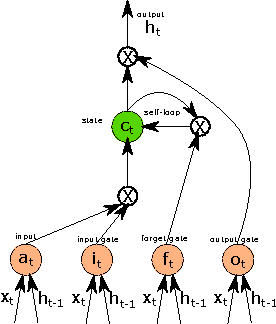
\includegraphics[width=0.6\linewidth]{figures/lingvist/lstm.pdf}
\caption[The long short-term memory cell]{A functional overview of the LSTM cell. The input~$x_t$ and the output of the previous timestep~$h_{t-1}$~are modulated by the input activation function~$f(x_t, x_{t-1}) = a_t$. The cell state is updated by $c_t = i_t \cdot a_t + f_t \cdot c_{t-1}$, such that the previous state of the cell $c_t$ is modulated by the forget gate $f_t$.}
\label{fig:lu_example}
\end{figure} 

Effectively, this means that on a per-user basis, the questions that are used to estimate the knowledge of a particular user are fed one-by-one into the LSTM cell, which creates a fixed-size representation of the user's knowledge, that is then mapped into the output space~$\vec{g}_\mathrm{pred}$. Between the LSTM layer and the output layer, we use a number of densely connected layers interleaved with dropout regularization~\cite{srivastava2014dropout} in order to approximate the knowledge decoding transformations between the knowledge representation and the output item space.

We use a RNN as opposed to a dense network working on a fixed-size input in order to be able to give accurate estimations of the user's knowledge before the full sequence is seen. Nevertheless, the RNN needs to be trained with a fixed input size~$N_{\mathrm{sequence}}$. The parameters to optimize in the model are the input, output and forget gate weights and biases and the weights of the dense layers connecting the LSTM output to the final output vector. As hyperparameters, we optimize the size of the LSTM layer, the number and size of the intermediate dense layers and the amount of dropout that is applied.

Care must be taken when computing loss function that is minimized in optimizing the weights. Since for any user, the known guess vector~$\vec{g}_\mathrm{true}$~, the prediction target, is sparse, we must compare only those prediction values for which the true value is known. Technically, we implement this by propagating the boolean mask of available answers as an auxiliary input along with the guess data and compute the binary cross-entropy loss only over available answers.

\subsection{Model architecture}
\label{sec:nlp_model_architecture}
In order to feed the~$(\mathrm{LU}, \mathrm{answer})$~pairs into the LSTM, we need to define an appropriate numerical representation of the LUs in the form of a fixed-length vector. As the set of all possible questions is known at training time, we could simply consider each LU as a unique symbol that can be embedded into a real vector space of dimension~$k$~by some appropriate function~$f(n) \Rightarrow \mathbb{R}^k$. The simplest approach would be to represent each LU in the "one-hot" encoding with~$k=n$, such that~$f_k(n) = \delta_{nk}$. This suffers from a dimensionality problem, as the number of LUs can in principle be arbitrarily large.

In our case, each LU is also a word, or more precisely a word pair in the source-target languages, thus we could use an existing word embedding such
as~\texttt{word2vec}~\cite{mikolov2013efficient} or~\texttt{GLOVE}~\cite{pennington2014glove} defined on a large corpus of text. These methods specify the embedding function based on contextual similarity. However, a predefined word embedding would limit the model to only be useful for word-based questions, making it difficult to use data from other types of learning activities.

Another option would be to derive the embedding directly as part of the neural network optimization procedure by using an embedding layer that reduces the dimensionality of the one-hot encoding. The advantage of this approach is that the embedding function~$f(n)$~can be optimized as part of the model, thus, the theoretical performance is the highest. This was the first approach we adopted and overall, it showed promising results. However, since over the lifetime of the model the items in LU set can change due to modifications to the course structure, we have investigated an encoding which is resilient to such changes and does not need re-optimization.

Instead of an optimized embedding described above, we may use random vectors to represent the questions. Using compressed sensing, we can reconstruct any d-dimensional k-sparse signal using random vectors that have at most~$r \simeq k\log d/k$~dimensions~\cite{baraniuk2007compressive}. In our case, the dimensionality is the number of individual LU items~($N \simeq 6000$) or symbols that we want to represent and the sparsity is~$k=1$~for a one-hot encoding, thus, a uniform random vector of length 4-5 would be sufficient to represent all the word pairs in the full course.

As mentioned above, the contents of the course may change over the lifetime of the model. Therefore, we wish to ensure that any new LU could be represented by the chosen embedding. We choose the random vector approach, as we can easily use the unique~\texttt{UUID4}-based identifiers of the LUs used in the internal database at Lingvist. We do this by mapping the 128 random bits of~\texttt{UUID4} to 16 random 8-bit floats in the range~$[-1, +1]$. With this method, it is straightforward to keep track of item (LU) to representation associations throughout the lifetime of the model, as they are always uniquely specified just by the item's identity. This practical arose when implementing the model in the production system at Lingvist. 

For each user, we take up to a fixed number~$N_{\mathrm{seq}} = 10\dots100$~of guesses as the input. These guesses are then represented as a~$N_{\mathrm{seq}} \times (r + 1)$~matrix, where~$r=16$~based on the compressed sensing arguments discussed above. Each row of the matrix corresponds to a tuple of the LU representation and the guess value~$g=\{0,1\}$. The output of the model is the~$n$-dimensional knowledge vector~$\vec{g}$, such that we predict the static knowledge of all LUs, based on a short guess sequence. The model is thus the following:

\begin{gather*}
\mathrm{sequence} = [(\mathrm{item}, \mathrm{guess}), (\mathrm{item}, \mathrm{guess}), \dots] \rightarrow \\
\rightarrow \mathbf{LSTM} \rightarrow \mathrm{encoded\ knowledge} \rightarrow \\ \rightarrow \mathrm{dense~layer} \rightarrow \cdots \rightarrow \mathrm{dense~layer} \rightarrow \\
\rightarrow \mathrm{dense\ output\ with\ sigmoid\ activation} \rightarrow \vec{g} 
\end{gather*}

\subsection{Optimization}
The loss function of a particular user~$m$~for the model optimization is based on a binary cross-entropy between the predicted knowledge and the true guess for all the items for which this user has provided answers. It has the form

\begin{equation}
L_m = \sum_{n \in \mathrm{ans}_m} \mathrm{H}(y_n, g_n)
\end{equation}
where~$\mathbf{y} = (y_n)$~is the predicted knowledge vector,~$g_n$~is the guess (prediction target) for a given item~$n$~in the set of answered items~$\mathrm{ans}_m$~for user~$m$. The binary cross-entropy between two vectors~$y_n\in[0,1]$~and~$g_n\in [0,1]$~is defined as

$$\mathrm{H}(y_n, g_n) = -[g_n \ln{y_n} + (1 - g_n)\ln{(1 - y_n)}].$$
It is related to the Kullback-Leibler (KL) divergence, defined over the true probability distribution~$g(x)$~and the assumed distribution~$h(x)$~as

\begin{equation}
\mathcal{D}_{\mathrm{KL}}(g||h) = \mathbb{E}_g \ln{\frac{g(x)}{h(x)}} = \int g(x) \ln{g(x)}\ \mathrm{d}x - \int g(x) \ln{h(x)}\ \mathrm{d}x \geq 0
\end{equation}
through~$\mathrm{H}(g,h) = \mathrm{H}(g) - \mathcal{D}_{\mathrm{KL}}(g||h)$~with~$\mathrm{H}(g) = -\mathbb{E}_g \log{g}$~being the Shannon entropy. In the case of binary discrimination, the distributions are defined by a single probability value~$g(1) = p$~and~$g(0) = 1 - p$, such that the Shannon entropy is maximal for $p=0.5$. The KL divergence is a discrepancy measure between the true and assumed distributions, which satisfies $\mathcal{D}_{\mathrm{KL}}(g||g) = 0$, but is not symmetric nor does it satisfy the triangle inequality, hence it is not a true distance measure. It can be shown that minimizing the KL divergence is equivalent to maximising the likelihood.

We optimize the model with respect to the loss function with random subsamples (minibatches) of 100 users for about 10-100 epochs with the Adam stochastic gradient descent optimizer over the whole dataset. The Adam method estimates first and second moments of the gradients of the loss function and uses it to adaptively update the parameter estimates~\cite{DBLP:journals/corr/KingmaB14}. The model was implemented using the tensorflow package~\cite{2016arXiv160304467A} and the optimization was performed on a single AWS \texttt{g2.2xlarge} instance, with an epoch time around~$\mathcal{O}(10~\mathrm{s})$.

\section{Results}
In this section, we will discuss the optimization studies of the model and the overall performance as estimated on held-out data.

\subsection{Studies of the RNN model}
In general, the model performance has only a mild dependence on the choice of hyperparameters, introduced in~\cref{sec:nlp_model}. Nevertheless, we scan the hyperparameter space by computing a cross-validated mean AUC at each point in a 5-dimensional space, consisting of the size of the LSTM layer, the size of the intermediate dense layers, the number of intermediate dense layers, the amount of dropout and the learning rate. We find that the hyper-parameter scan prefers the encoding by the LSTM to be rather small, around 32 to 64 units, and the intermediate dense layers are preferred to be small (128-256) and deep (3-4 layers). The final optimized loss function is shown on~\cref{fig:loss}, where we see from the loss on the training set that the model has sufficient generality to be able to fit features of the data, with the performance on the held-out test set being still acceptable after 10-15 epochs.

\begin{figure}[ht]
\centering
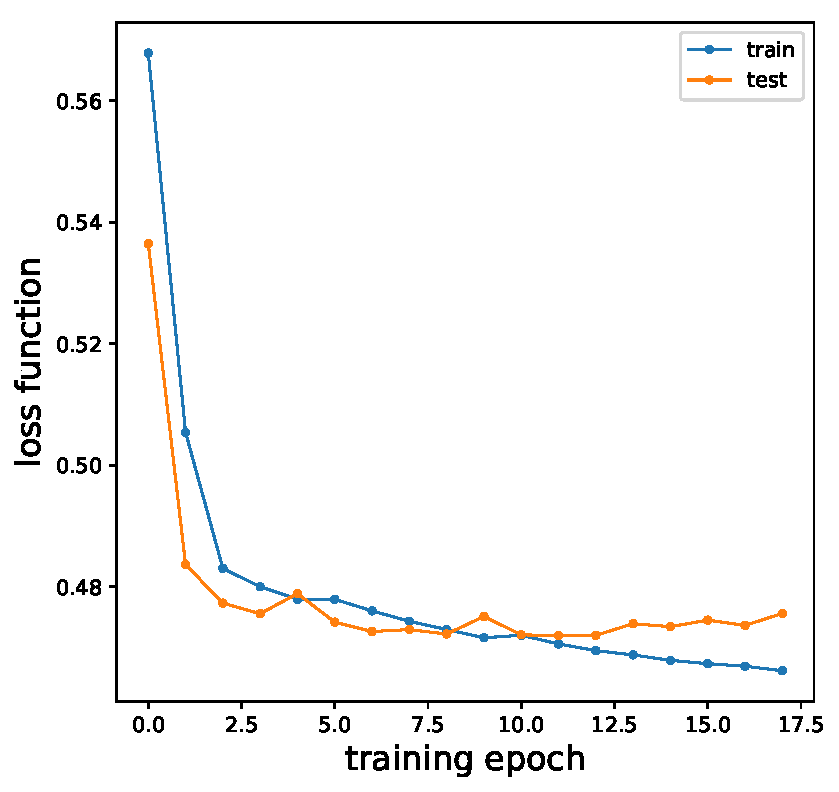
\includegraphics[width=0.5\linewidth]{figures/lingvist/loss.pdf}
\caption[Loss function for the knowledge estimation model]{The loss function of the final optimization of the model. The loss on the training set is shown in blue, the validation set in orange. In general, we see a relatively good convergence of the model after approximately 10-15 optimization epochs.} 
\label{fig:loss} 
\end{figure} 

One of the more important free parameters of the model is the length of the input guess sequence~$N_{\mathrm{seq}}$, introduced in~\cref{sec:nlp_model_architecture}. While RNN-type networks can work with an input of arbitrary length, there is a clear trade-off between the amount of information provided to the model vs. the amount it needs to predict.
We have studied how this affects the performance of the model by retraining the model on the same dataset, selecting up to~$N_{\mathrm{seq}}$~guesses for each user. In order not to bias the analysis, as users with a different number of guesses may have different knowledge characteristics, we train on the same underlying data where users have at least~$N_{\mathrm{seq}} = 100$~guesses, masking the additional sequence elements. As expected, the model performs better with longer sequences, as more information is provided about the user. We observe a roughly linear relationship between the AUC and the guess sequence length, as can be seen on~\cref{fig:seq_length}.

\begin{figure}[ht]
\centering
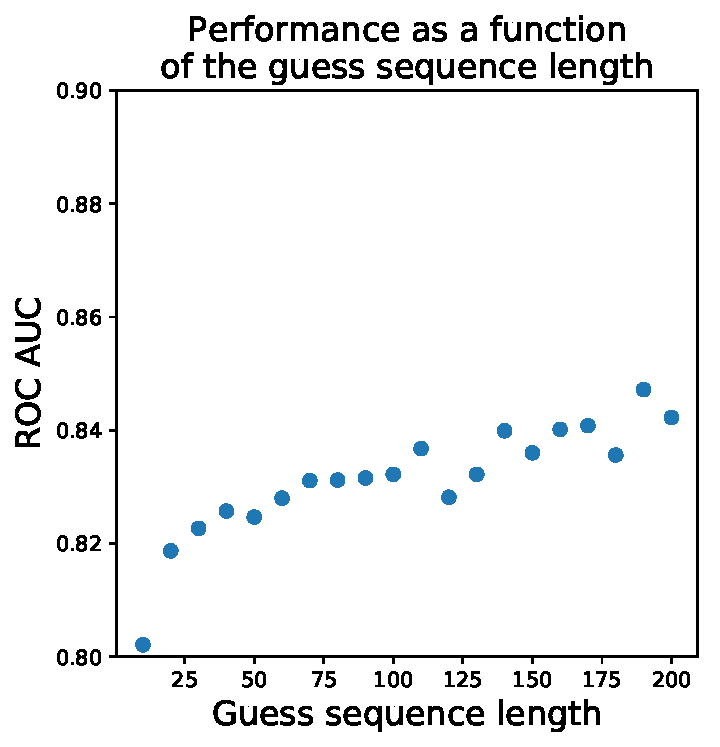
\includegraphics[width=0.5\linewidth]{figures/lingvist/seq_length.pdf}
\caption[Performance as a function of sequence length.]{Performance of the model as a function of the guess sequence length. For each point, we use only up to~$N_{\mathrm{sequence}}$~guesses from all users as the input to the model. The model is trained from scratch on the full dataset and evaluated in the same way for all cases.} 
\label{fig:seq_length} 
\end{figure} 

Additionally, we have studied how the amount of training statistics affects the performance of the model. Interestingly, we see that with even as few as 1000 users, the model is able to approximate the knowledge characteristics of an average user. In general, adding more data improves the performance more significantly for words for which there are very few answers provided, as can be seen on~\cref{fig:statistics}. Adding more data improves the model performance, especially for words with very low answer rates.

\begin{figure}[ht]
\centering
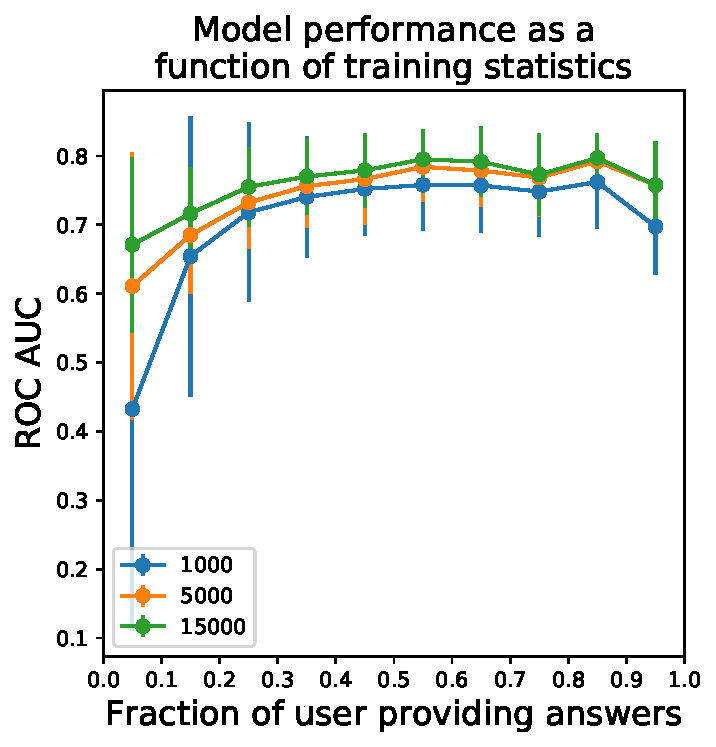
\includegraphics[width=0.5\linewidth]{figures/lingvist/statistics.pdf}
\caption[The effect of training statistics on the model performance.]{The effect of the amount of training data on the model performance We investigate 3 cases: 1000 users, 5000 users, 15000 users (full dataset) and plot the performance characteristics of the model (ROC AUC), averaged over words that have a certain fraction of users providing answers. Overall, we see that the model performance increases significantly for words with few answers when adding training data.}
\label{fig:statistics}
\end{figure}

\subsection{Discussion}

As a first step, we compare the average performance of the model over all guesses to the reference toy model. We show the average performance of the RNN model on~\cref{fig:roc} on a held-out dataset that was not seen during optimization. In general, we see that the RNN model is more accurate than the average model, with the average true positive rate improving from 0.38 to 0.54 at an average false positive rate of 0.1 for the trial-weighted case, an improvement of about 40\% in efficiency. This conclusion also holds if all LUs are given equal weight. This is not surprising, as the reference model has no discriminating information about the individual users or LUs. This increase in efficiency directly translates into reduced learning time, as the LUs correctly predicted can be defocused in the study period without losing the coverage of the course.

\begin{figure}[ht]
\centering
\begin{tabular}{cc}
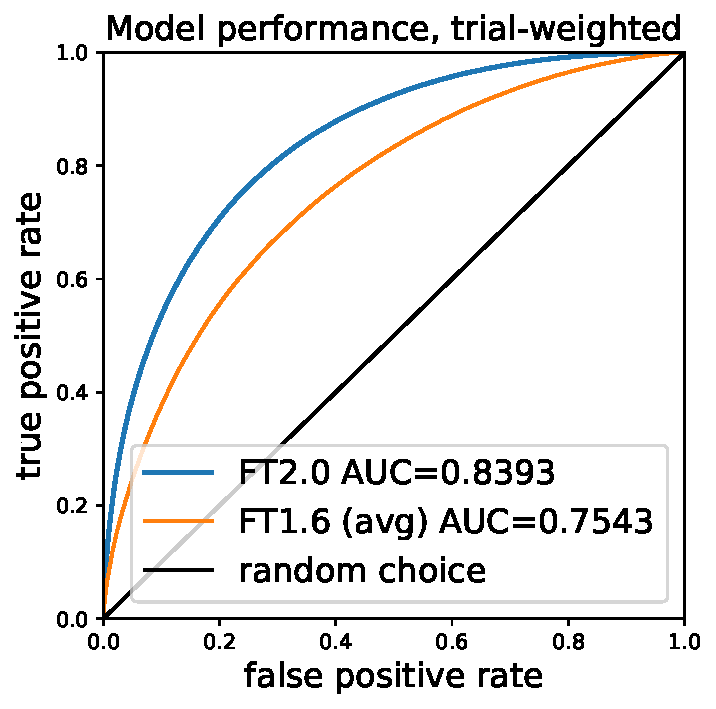
\includegraphics[width=0.4\linewidth]{figures/lingvist/roc_trial.pdf} &
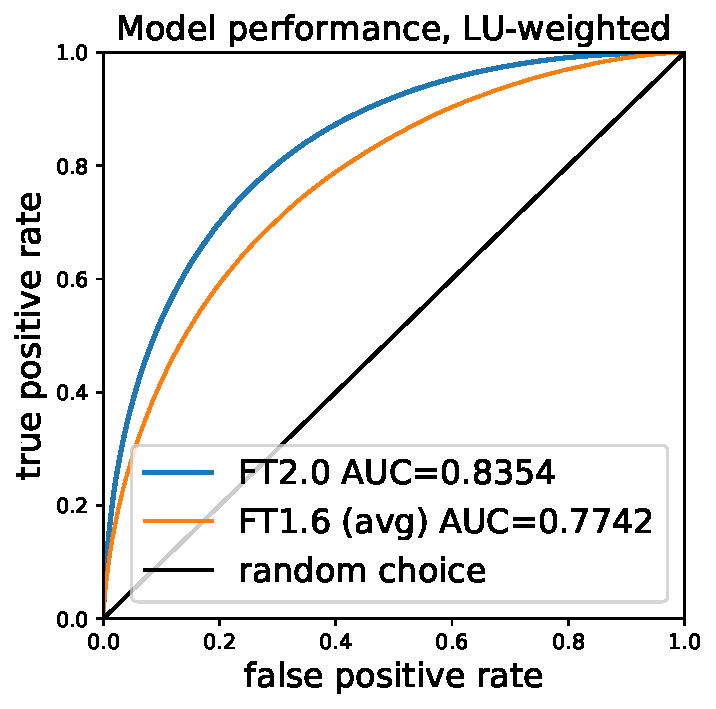
\includegraphics[width=0.4\linewidth]{figures/lingvist/roc_lu.pdf} \\
\end{tabular}
\caption[Overall knowledge estimation model performance]{Overall average performance of the model, as characterised by the receiver operating characteristic (false positive to true positive rate curve) area under curve (ROC AUC). On the left, we show the average treating all trials equally, on the right, the average by weighting trials such that each LU is treated equally. We see that the RNN model (blue) outperforms the average model (orange).} 
\label{fig:roc} 
\end{figure} 

Furthermore, we study some first-order statistics of the predictions, namely the per-user and per-LU averages. In a very simple model, each user (LU) can be characterized by their average correct rate, treating all LUs (users) as equal. More sophisticated treatments based on item response theory would also be possible, where the skills assigned to users and difficulties assigned to items are determined using a maximum likelihood procedure~\cite{embretson2013item}. On~\cref{fig:user_lu_correct_rate} we see that the average per-LU and per-user correct rates are also reproduced to a good degree by the model, with linear correlation coefficients above~$90\%$. We can see that the correct rate for users and LUs with a low (high) average correct rate are slightly under (over) estimated. This could result from the model not having enough counterexamples to sufficiently learn the probability distribution~$p(\vec{g})$~for very simple or difficult LUs and users with very low or high correct rate. We take this as an example that the model is able to summarize the user and LU population and approximate the mean correct rates.

\begin{figure}[ht]
\centering
\begin{tabular}{cc}
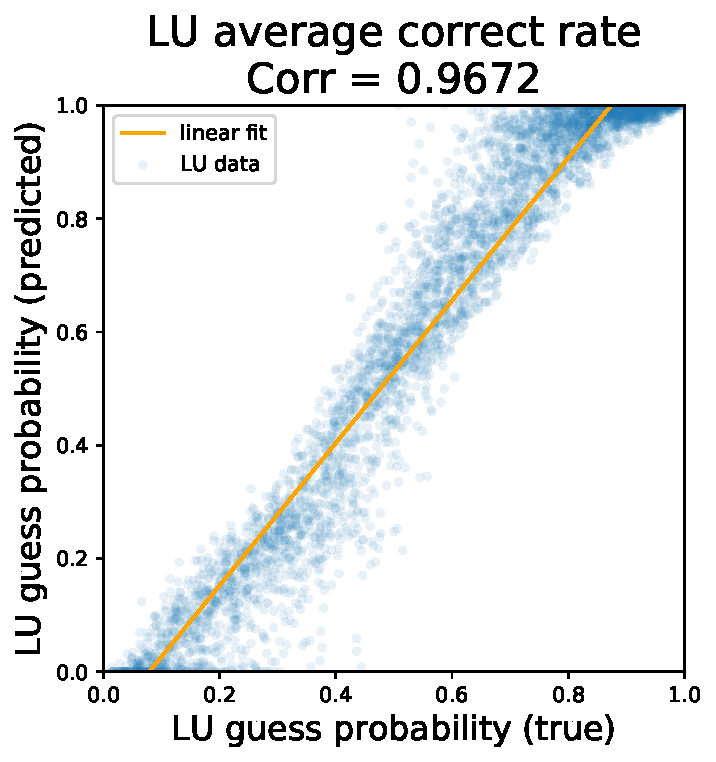
\includegraphics[width=0.4\linewidth]{figures/lingvist/lu_correct_rate.pdf} &
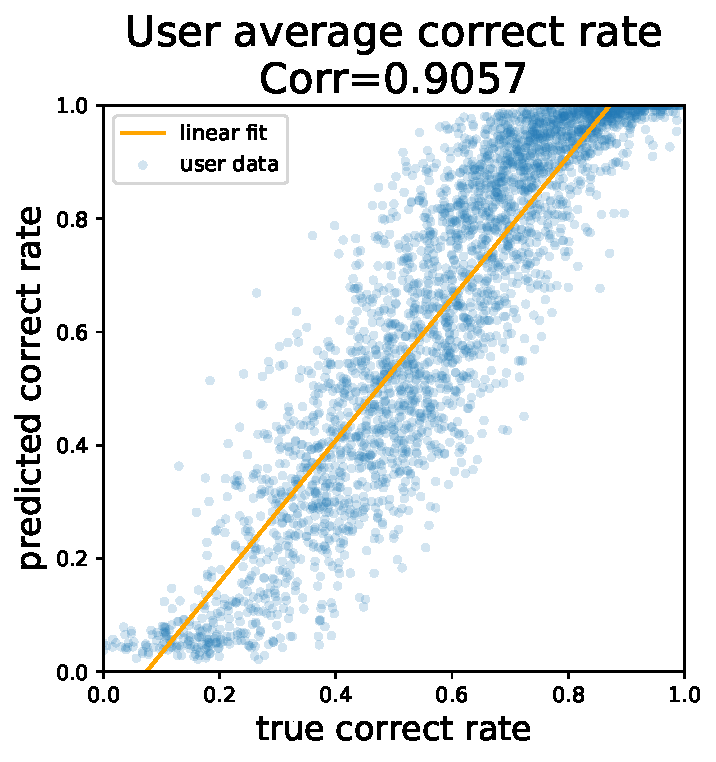
\includegraphics[width=0.4\linewidth]{figures/lingvist/user_correct_rate.pdf} \\
\end{tabular}
\caption[Predicted vs. true average guess rate]{Predicted vs. true average guess rate by LU (left) and user (right). We see that the model performs best for LUs which have a true correct rate around 50\%, with slight underestimation at low correct rates and overestimation at high true correct rates.}
\label{fig:user_lu_correct_rate}
\end{figure}

We can further study the average performance of the model on a per-LU, per-user basis as a function of number of guesses per LU. On~\cref{fig:lu_roc_prio} we see that the overall performance of the model is strongly dependent on how many guess attempts a given LU has, with the average ROC AUC dropping significantly for rarer LUs. This performance degradation is expected, as we can see from~\cref{fig:user_lu_distribution} that the number of answers per word drops steeply going further in the course, reflecting that this model was trained treating each trial equivalently. With increasing guess statistics, it may be worthwhile to investigate a re-weighting or re-sampling of the trials such that words that have fewer trials have a higher weight and would thus still be optimized for in the training. This trend also introduces a natural cut-off in terms of when the predictions from the model are no longer considered reliable at a priority index of around 4000 for LUs. The priority index arises from an ordering of the LUs by when they appear in the course on average and can simply be considered a specific way to order the LUs.

\begin{figure}[ht]
\centering
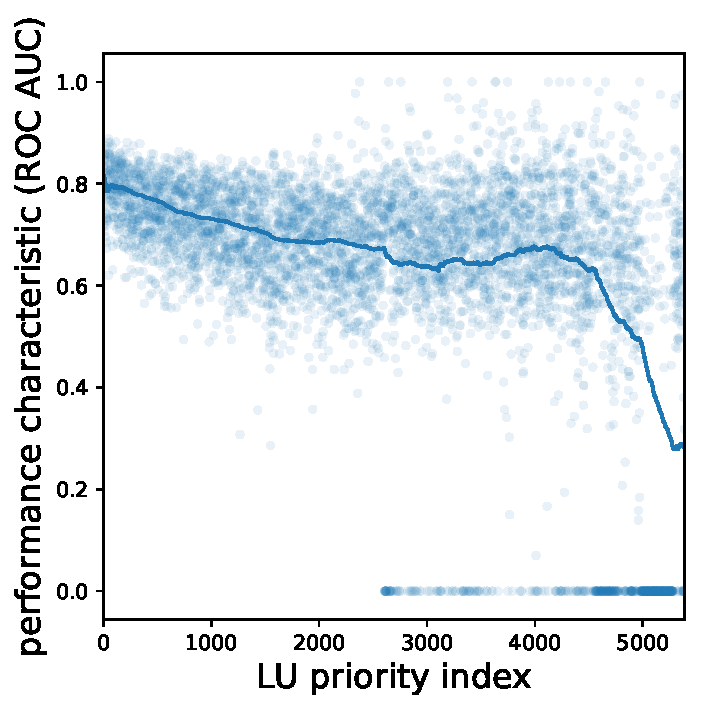
\includegraphics[width=0.5\linewidth]{figures/lingvist/lu_roc_prio.pdf}
\caption[Performance of knowledge estimation as a function of LU priority.]{The performance characteristic (ROC AUC) as a function of lexical unit priority index. The priority index is a monotonously growing index that roughly corresponds to the order in which words are shown to users, with lower indices being shown earlier and more often.}
\label{fig:lu_roc_prio}
\end{figure}

We further study the performance as a function of the LU average guess rate, which can be interpreted as the LU difficulty. We see on~\cref{fig:lu_roc_guess_proba} that the performance of the model is broadly similar over a wide range of difficulties. For words that are very easy or difficult, the variance in the trained model is considerable, since the model has less counterexamples for optimization. Furthermore, we see that the the LUs with vanishing performance all have 0 correct guesses in data, meaning they can be excluded from the predictions.

\begin{figure}[ht]
\centering
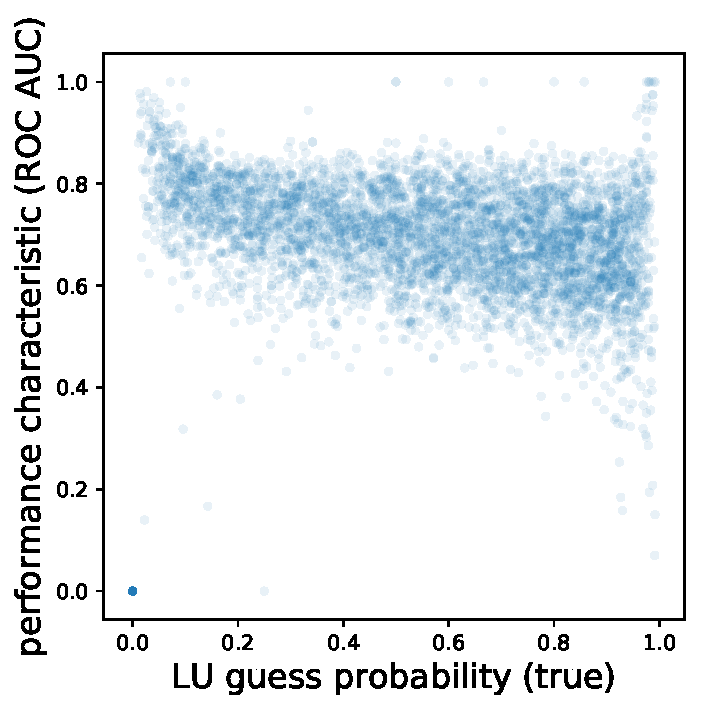
\includegraphics[width=0.5\linewidth]{figures/lingvist/lu_roc_guess_proba.pdf}
\caption[Model performance on a per-LU basis as a function of average LU guess probability.]{The performance of the model on a per-word basis as a function of the guess probability (prior difficulty) of the word. We see that for words with very high or low guess probability, the variance of the model is significant, resulting from few training examples.}
\label{fig:lu_roc_guess_proba}
\end{figure}

\subsubsection{Prediction uncertainty}
We have also investigated the prediction uncertainty arising from the model. In particular, for a word that is predicted to be known at a knowledge likelihood of~$y_m=0.9$, as an example, how certain is the model of this prediction and how much would it vary if the input sequence changed slightly? For neural networks, it has been shown that using dropout in the evaluation phase is a good approximation for the inherent prediction uncertainty~\cite{gal2016dropout}. On~\cref{fig:uncertainty}, we can see the evaluated uncertainty of the guess probability using 10 dropout rounds, compared to the data, in terms of the running mean of the average correct rate as a function of the LU priority index. It is interesting to see that the~$3\sigma$~confidence interval around the predicted mean covers the data, however, the predicted mean generally trends lower than the true guess probability.

\begin{figure}[ht]
\centering
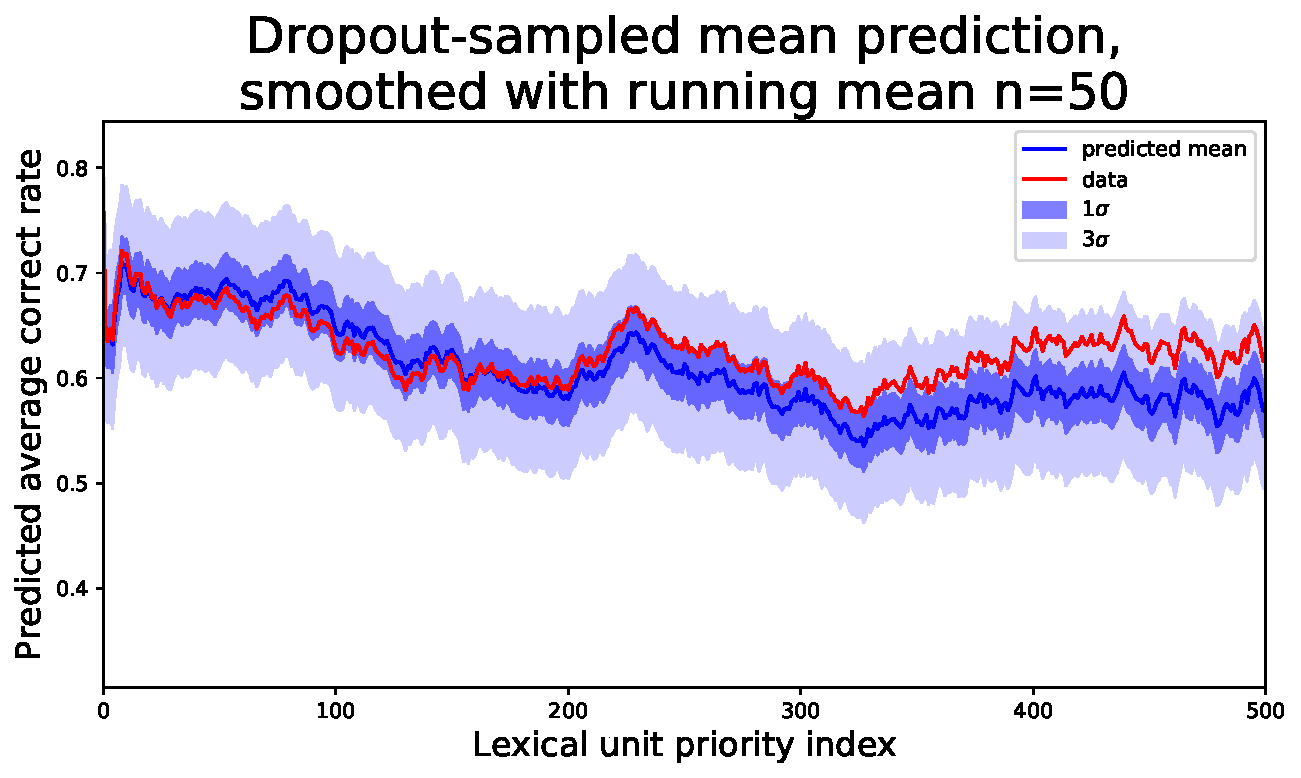
\includegraphics[width=1.0\linewidth]{figures/lingvist/uncertainty.pdf}
\caption[The sensitivity estimation of the model using dropout sampling.]{The predicted (blue) and true (red) guess probability as a function of LU priority index for the first 500 LUs. We see that the prediction is generally sufficiently close to the true mean correct rate, but trends somewhat lower than the data.}
\label{fig:uncertainty}
\end{figure}

\subsection{Future work}
As possible future improvements, extending the information in the LU feature vector beyond a random representation may prove to be a straightforward way to improve the performance of the model. In particular, the random representation could be augmented with features such as difficulty or context based on expert labelling. This is particularly important, as the LUs are embedded in sentences, so context priming effects could be significant~\cite{elgort2011deliberate}.

Additionally, the DKT approach was originally conceived for time-dependent knowledge modelling and the current framework is naturally amenable to predicting the behaviour of the guess sequences in time, such that effects of acquisition and forgetting could naturally be incorporated.

Furthermore, the current model works only on a single language pair, but it could easily be extended to multiple simultaneous languages by adding language data to the source representation vector and decoding the internal knowledge representation into different target language spaces. This would allow training a single model on all language pairs simultaneously, which could help bootstrapping new courses that don't yet have enough user interaction data. 

\subsubsection{Interpretable models}
Having optimized a model that is capable of estimating the knowledge vector~$\vec{g}$~based on a subset of guesses, it is interesting to study the explanatory factors of that model. In general, explaining the decisions or predictions of complex "black box" models is a topic of intense research activity~\cite{2017arXiv170808296S}. Recently, locally interpretable linear models (LIME) have been proposed as a way of explaining the features a model makes use of for particular prediction outcomes~\cite{ribeiro2016should}. In the LIME approach, any classifier or regressor predictions can be explained in a locally faithful way by fitting local linear approximations to the decision. We have used the method to validate our optimized vocabulary model on a few examples and see that it uses guess information in an intuitively correct way, as can be see on~\cref{fig:lime}. We mention this as a possible direction for future research, as understanding the factors in a prediction by a complex model is an essential step in validation.

\begin{figure}[ht]
\label{fig:lime}
\centering
\begin{tabular}{cc}
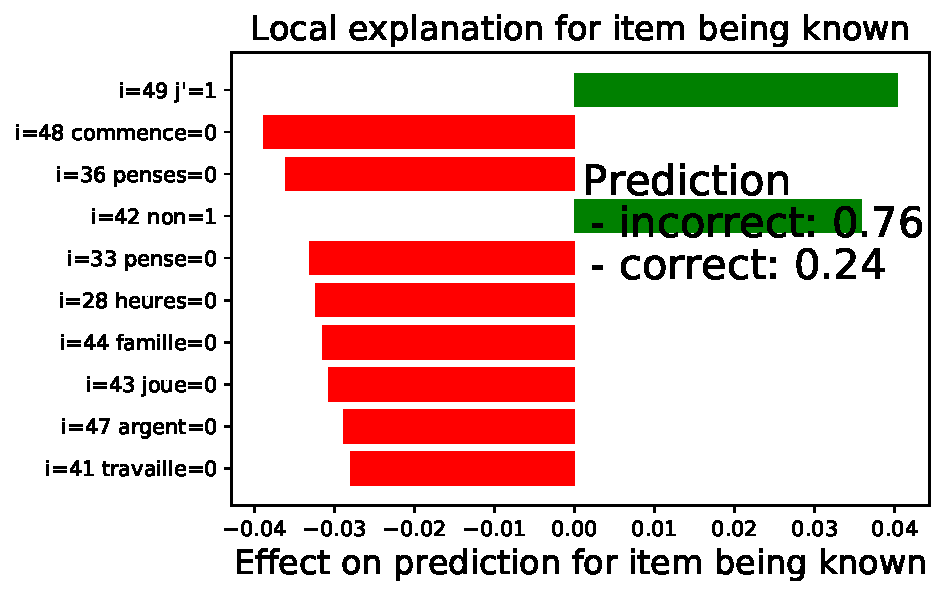
\includegraphics[width=0.4\linewidth]{figures/lingvist/lime_pos.pdf} &
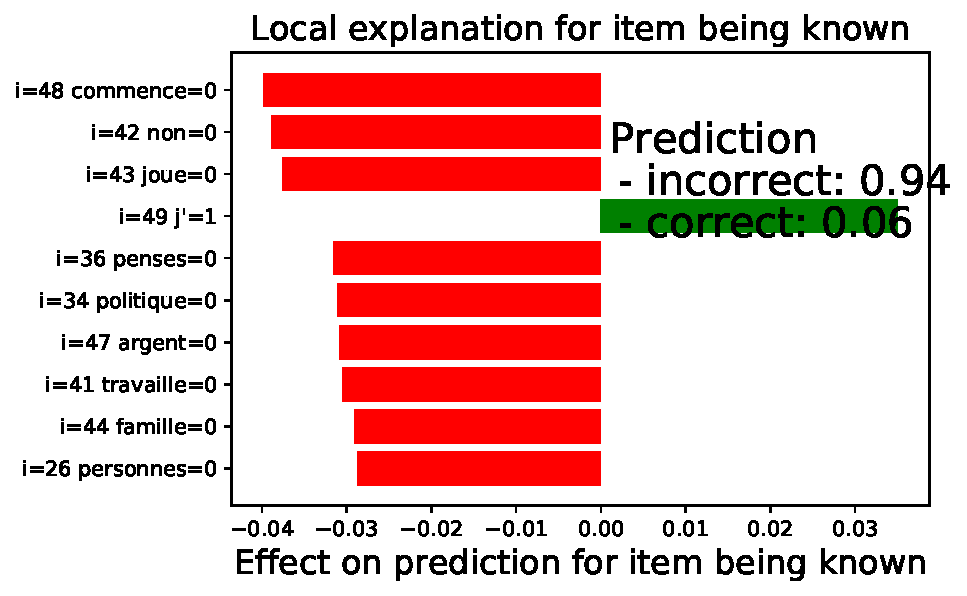
\includegraphics[width=0.4\linewidth]{figures/lingvist/lime_neg.pdf} \\
\end{tabular}
\caption[Local explanations of the model prediction]{Local explanations for a word that was known (left) and not known (right). In the case where the word was known, the algorithm predicts the knowledge likelihood to be~$g = 0.24$, based on the correct guesses of the LUs \textit{j'} and \textit{non}, but incorrect guesses for most other words in the trial set. In the case where the word was not known on the right, the model predicts the guess likelihood to be~$g = 0.06$~based on incorrect guesses for most words. We see that incorrect guesses ($=0$, red) tend to affect the prediction in a negative way, whereas correct guesses ($=1$, green) tend to reinforce the knowledge, as would be expected.}
\end{figure}


\section{Summary}
We have shown that by formulating the problem of predicting existing knowledge as a sequence-to-vector binary classification problem, RNNs present a simple and flexible solution applicable to a wide variety of cases. This method outperformed the existing reference implementation at Lingvist by about 45\% in terms of true positive rate at a fixed false positive rate. In order to achieve this result, we formalized the reference model based on average guess accuracies and formulated the vocabulary prediction problem as binary classification. We have found that sparse coding from random bits in database identifiers can be used to represent categorical items in a practical and resilient fashion.

Moreover, we have seen that a single flexible model architecture based on recursive neural networks is able to predict knowledge probabilities of thousands of words based on just a small amount of randomly chosen guesses. The RNN model is easily extensible, should more information about LUs or users become available. In particular, we see extension to predicting knowledge in multiple languages simultaneously or incorporating time-dependent information as possible future improvements.

Furthermore, we have studied the reliability of the predictions by evaluating the sensitivity of the model to the inputs using a sampling technique which allows to attach uncertainties to predictions and by deriving locally-interpretable models around predictions. Using this sensitivity analysis in HEP, where multivariate predictions are commonplace, would allow the reliability of these results to be studied from a new perspective.

Overall, in cases where the amount of available data is significant but the underlying theory is not well known from first principles, such as language acquisition, the use of ML for modelling and prediction tasks can provide significant advantages in terms of flexibility and speed over approaches that require expert annotations, such as Bayesian Knowledge Tracing.